\section{Evaluation}

We evaluated the timing compartments architecture using the gem5 architectural 
simulator~\cite{gem5} integrated with the DRAMSim2~\cite{DRAMSim2} 
memory simulator. Our experiments use multiprogram workloads 
comprised of groups of SPEC2006 benchmarks compiled for the ARM ISA. 

Table~\ref{tab:config} shows our system configuration.
The cores use the gem5 ``O3`` out-of-order core model which runs at 2GHz. 
Each core has private 32KB L1 instruction and data caches, and private 256KB L2 
cache. The cores share a 4MB L3 cache. We derived cache configuration 
parameters from the Intel Xeon E3-1220L, which is a two core architecture used 
by Amazon EC2. In DRAMSim2, we simulate a 667MHz 2GB DDR3 memory. The 
interconnects in the simulator runs at 1GHz. Unless specified otherwise, each experiment is 
fastforwarded for 1 billion instructions, and run for 100 million 
instructions. We will first describe our security evaluation and then show
the performance evaluation.

\begin{table}
    \caption{Simulator configuration parameters.}
    \centering
    \begin{tabular}{|l|l|l|r|}
        \hline
        \multicolumn{3}{|l|}{gem5 core model} & ``O3''        \\\hline
        \multicolumn{3}{|l|}{CPU Clock}    & 2GHz             \\\hline
        \hline
        \multicolumn{2}{|l|}{Memory}             & 2GB    & 667MHz  \\\hline
        \hline
        \multicolumn{3}{|l|}{Network Clock}      & 1GHz \\\hline
        \hline
        L1d / L1i  & 32kB   & 2-way  & 2 cycles\\\hline
        L2         & 256kB  & 8-way  & 7 cycles \\\hline
        L3         & 4MB    & 16-way & 17 cycles  \\\hline
    \end{tabular}
    \label{tab:config}
\end{table}

\subsection{Security Evaluation}

To experimentally evaluate the security of the timing channel protection in our architecture,
we use a two-core system with two timing compartments, TC0 and TC1, running
concurrently. The protection policy is configured to disallow any timing channel between
the two compartments.
If the number of cycles required to execute certain number of instructions 
for a particular benchmark running on TC0 depends on which benchmark is running on 
TC1, it indicates timing interference exists.% that can be exploited to leak information about TC0. 
A secure scheme should guarantee the benchmark running in TC0 always uses the same number of cycles
to finish regardless of which benchmark TC1 is running. 

Using the rule above, we evaluated the security of our architecture by running a fixed benchmark
on TC0 while varying the benchmark on TC1. Then we compared the total execution time for the fixed
benchmark in different runs. We evaluated our architecture as well as the baseline insecure architecture 
which does not implement any protection. As expected, the results for
the baseline show the execution time of the fixed benchmark (TC0) changes significantly depending on 
the benchmark in TC1, indicating timing channels exist between the two cores. On the other hand,
the results for our architecture show no execution time difference for the fixed benchmark when
running 1 million instructions. 
When running 10 million instructions, a small number of benchmarks in TC0
showed an execution time difference of two cycles. We believe this is a minor bug in our
implementation, and we are working on eliminating them.

\subsection{Performance Evaluation}

Copmared to the baseline scheme, our timing compartment architecture uses static partitioning and time multplexing
in the shared hardware resources, which can introduce performance overhead due to
underutilization. To evaluate the performance overhead, we ran the SPEC2006 benchmarks in a pair of two, and
measured the execution time of the fixed benchmark in TC0. The memory intensity of the benchmarks are shown
in Figure~\ref{fig:memstudy}. For the baseline architecture, we calculate the average execution time of the fixed benchmark
by averaging the runs with different benchmarks in TC1. This is due to the fact that the timing of the fixed
benchmarks changes in different runs. 
In our scheme, the execution time of TC0 stays constant no matter which benchmark runs in TC1.

\begin{figure}
    \begin{center}
        \includegraphics[width=3.46in]{figs/memstudy.pdf}
        \caption{Memory intensity of SPEC2006 benchmarks.}
        \label{fig:memstudy}
    \end{center}
\end{figure}

The performance overhead results are shown in Figure~\ref{fig:performance}. The Y axis shows the 
execution time normalized to the baseline. As can be seen, the performance overhead is quite low
for the benchmarks with low memory intensity. For libquantum and mcf, the performance overhead is about 
25\%, which is still quite low.
%compared to previous full system protection approaches which incurs serveral
%times of overhead. 
The results show that the timing compartments are viable in today's microprocessors,
especially for applications that require high assurance for software isolation.

\begin{figure}
    \begin{center}
        \includegraphics[width=3.46in]{figs/performance.pdf}
        \caption{Performance overhead for 2 TCs.}
        \label{fig:performance}
    \end{center}
\end{figure}

The performance overhead is likely to increase as the number of timing compartment scales up.
To study the impact of the number of timing compartments,
we evaluated the performance overhead with four timing
compartments on a 4-core processor, each occupying one core and private L1 and L2 caches. 
They share a 4MB L3 cache. The performance
overhead is shown in Figure~\ref{fig:scalability}. 
We show two bars for the baseline. One bar represents the performance when a 
benchmark is running with three copies of astar ({astar, astar, astar}), and the other bar represents the performance when running with mcf ({mcf, mcf, mcf}). 
This
is because the baseline scheme shows different execution time when running with different benchmarks.
We
chose astar and mcf because they represent the least and most memory intensive benchmarks in our benchmark
suites. We also show the performance with four timing compartments. All results are normalized to the baseline when running
with astar. Again, libquantum and mcf show the highest overhead, 63\% and 79\% respectively, because of their 
high memory intensity. 
The results suggest that the overhead of timing compartments is rather insensitive
to the number of timing compartments for compute-bound applications. For memory-intensive
applications, the overhead can increase noticeably. However, the results still suggest
that running multiple timing compartments sharing the same processor provides better
overall efficiency compared to requiring dedicated machines.


\begin{figure}
    \begin{center}
        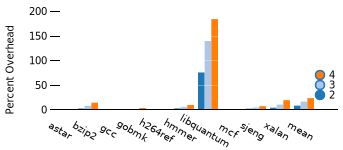
\includegraphics[width=3.46in]{figs/scalability.pdf}
        \caption{Performance overhead for 4 TCs.}
        \label{fig:scalability}
    \end{center}
\end{figure}

While future multi-core systems are likely to have a large number of processing cores,
we note that many security applications will not require many timing compartments to
be used concurrently. For example, the BYOD application only requires two TCs no matter
how many cores exist in the system. Similarly, in the high-assurance cloud computing
scenario, the cloud provider can limit the number of high-assurance virtual machines
that can be located on each physical system while increasing the system utilization 
by co-locating non-secure virtual machines with high-assurance ones.



